

\tikzset{every picture/.style={line width=0.75pt}} %set default line width to 0.75pt        

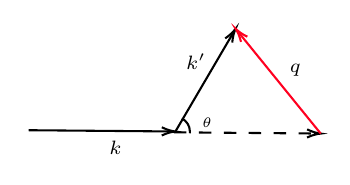
\begin{tikzpicture}[x=0.75pt,y=0.75pt,yscale=-1,xscale=1]
%uncomment if require: \path (0,583); %set diagram left start at 0, and has height of 583

%Straight Lines [id:da47989121087390596] 
\draw    (130,160) -- (198.68,160.6) ;
\draw [shift={(200.68,160.62)}, rotate = 180.5] [color={rgb, 255:red, 0; green, 0; blue, 0 }  ][line width=0.75]    (6.56,-1.97) .. controls (4.17,-0.84) and (1.99,-0.18) .. (0,0) .. controls (1.99,0.18) and (4.17,0.84) .. (6.56,1.97)   ;
%Straight Lines [id:da5560514482873335] 
\draw    (200.68,160.62) -- (228.67,112.83) ;
\draw [shift={(229.68,111.1)}, rotate = 120.36] [color={rgb, 255:red, 0; green, 0; blue, 0 }  ][line width=0.75]    (6.56,-1.97) .. controls (4.17,-0.84) and (1.99,-0.18) .. (0,0) .. controls (1.99,0.18) and (4.17,0.84) .. (6.56,1.97)   ;
%Straight Lines [id:da8910385526119278] 
\draw  [dash pattern={on 4.5pt off 4.5pt}]  (200,161) -- (268.68,161.6) ;
\draw [shift={(270.68,161.62)}, rotate = 180.5] [color={rgb, 255:red, 0; green, 0; blue, 0 }  ][line width=0.75]    (6.56,-1.97) .. controls (4.17,-0.84) and (1.99,-0.18) .. (0,0) .. controls (1.99,0.18) and (4.17,0.84) .. (6.56,1.97)   ;
%Straight Lines [id:da6496315176862661] 
\draw [color={rgb, 255:red, 255; green, 0; blue, 32 }  ,draw opacity=1 ]   (270.68,161.62) -- (230.94,112.65) ;
\draw [shift={(229.68,111.1)}, rotate = 50.94] [color={rgb, 255:red, 255; green, 0; blue, 32 }  ,draw opacity=1 ][line width=0.75]    (6.56,-1.97) .. controls (4.17,-0.84) and (1.99,-0.18) .. (0,0) .. controls (1.99,0.18) and (4.17,0.84) .. (6.56,1.97)   ;
%Shape: Arc [id:dp644522715932185] 
\draw  [draw opacity=0] (203.8,154.37) .. controls (206.09,155.52) and (207.66,157.88) .. (207.66,160.62) .. controls (207.66,160.9) and (207.64,161.19) .. (207.61,161.47) -- (200.68,160.62) -- cycle ; \draw   (203.8,154.37) .. controls (206.09,155.52) and (207.66,157.88) .. (207.66,160.62) .. controls (207.66,160.9) and (207.64,161.19) .. (207.61,161.47) ;  

% Text Node
\draw (167.34,163.71) node [anchor=north west][inner sep=0.75pt]  [font=\scriptsize]  {$\vb{k}$};
% Text Node
\draw (204.34,121.71) node [anchor=north west][inner sep=0.75pt]  [font=\scriptsize]  {$\vb{k}'$};
% Text Node
\draw (254.34,126.71) node [anchor=north west][inner sep=0.75pt]  [font=\scriptsize]  {$\vb{q}$};
% Text Node
\draw (212,152.4) node [anchor=north west][inner sep=0.75pt]  [font=\tiny]  {$\theta$};


\end{tikzpicture}
